\documentclass[aspectratio=169, 10pt]{beamer}
\usepackage[spanish,es-tabla]{babel}
\usepackage[utf8]{inputenc}
\usepackage{graphicx}
\usepackage{booktabs}
\usepackage{amsmath,amssymb}
\usepackage{tikz}
\usepackage{microtype}

% Directorio de figuras
\graphicspath{{../../resultados/figuras/}{../../resultados/}{../../Archivos/images/}}

% Configuración del tema y colores institucionales (Externado de Colombia)
\usetheme{Madrid}
\usecolortheme{default}

\definecolor{ExternadoAzul}{RGB}{0, 45, 98}        % Azul corporativo
\definecolor{ExternadoDorado}{RGB}{197, 155, 39}    % Dorado institucional
\definecolor{GrisOscuro}{RGB}{40, 40, 40}
\definecolor{FondoClaro}{RGB}{248, 249, 250}

\setbeamercolor{palette primary}{bg=ExternadoAzul,fg=white}
\setbeamercolor{palette secondary}{bg=ExternadoAzul!85!black,fg=white}
\setbeamercolor{palette tertiary}{bg=ExternadoAzul!70!black,fg=white}
\setbeamercolor{titlelike}{parent=palette primary,fg=ExternadoAzul}
\setbeamercolor{frametitle}{bg=ExternadoAzul,fg=white}
\setbeamercolor{structure}{fg=ExternadoAzul}
\setbeamercolor{block title}{bg=ExternadoAzul,fg=white}
\setbeamercolor{block body}{bg=FondoClaro,fg=GrisOscuro}

\setbeamertemplate{navigation symbols}{}
\setbeamertemplate{headline}{}

% Pie de página personalizado
\setbeamertemplate{footline}{
  \leavevmode%
  \hbox{%
  \begin{beamercolorbox}[wd=.333333\paperwidth,ht=2.25ex,dp=1ex,center]{author in head/foot}%
    \usebeamerfont{author in head/foot}Torres $\cdot$ López $\cdot$ Figueroa
  \end{beamercolorbox}%
  \begin{beamercolorbox}[wd=.333333\paperwidth,ht=2.25ex,dp=1ex,center]{title in head/foot}%
    \usebeamerfont{title in head/foot}Machine Learning II (2026-II)
  \end{beamercolorbox}%
  \begin{beamercolorbox}[wd=.333333\paperwidth,ht=2.25ex,dp=1ex,right]{date in head/foot}%
    \usebeamerfont{date in head/foot}Externado \hspace*{2em} \insertframenumber{} / \inserttotalframenumber \hspace*{2ex} 
  \end{beamercolorbox}}%
  \vskip0pt%
}

% -------------------------------------------------------------
% METADATOS DE LA PRESENTACIÓN
% -------------------------------------------------------------
\title[\textbf{SVM y Normalización en Deserción}]{\textbf{\Large Máquinas de Soporte Vectorial para la Predicción Temprana de Deserción Estudiantil Universitaria}}
\subtitle{\large Evaluación del Impacto de la Normalización bajo Metodología SPADIES 3.0}

\author[\textbf{Torres, López, Figueroa}]{\textbf{Arnold Santiago Torres Anzola} \\ \textbf{Sara López Chavarro} \\ \textbf{Nicolás Figueroa Salgado}}

\institute[\textbf{U. Externado}]{\small Universidad Externado de Colombia \\ Departamento de Matemáticas — Pregrado en Ciencia de Datos}
\date{Noviembre de 2026}

\begin{document}

% =============================================================
% SLIDE 1: PORTADA Y ARTÍCULO BASE DE REFERENCIA
% =============================================================
\begin{frame}[plain]
    \titlepage
    \begin{center}
        \footnotesize \textbf{Artículo Base de Referencia:} Boteju, G., Tang, L., \& Scott Brown, M. (IEEE BigData, 2024). \textit{Support Vector Machine for Predicting Student Dropout Under Different Normalization Methods}.
    \end{center}
\end{frame}

% =============================================================
% SLIDE 2: DATOS Y CONTEXTO NACIONAL (SPADIES 3.0)
% =============================================================
\begin{frame}{1. Estrategia de Datos: Fundamentación SPADIES 3.0 y EDA}
    \begin{columns}[T]
        % Columna Izquierda: Puntos clave
        \begin{column}{0.48\textwidth}
            \begin{block}{\textbf{Dataset y Formulación Multiclase}}
                \begin{itemize}\small
                    \item \textbf{Cohorte:} 11,500 estudiantes, 21 variables predictoras (académicas, socioeconómicas e institucionales).
                    \item \textbf{3 Estados Reales (SPADIES 3.0 - MEN):}
                    \begin{itemize}\footnotesize
                        \item \textbf{En curso (44.7\%):} Avance regular (5,137 est.).
                        \item \textbf{Desertor (33.6\%):} Retiro $\ge 2$ semestres (3,863 est.).
                        \item \textbf{Graduado (21.7\%):} Culminación exitosa (2,500 est.).
                    \end{itemize}
                \end{itemize}
            \end{block}
            
            \begin{block}{\textbf{Hallazgo Estadístico Clave: No Linealidad}}
                \begin{itemize}\small
                    \item $\text{Spearman} > \text{Pearson}$ en \texttt{promedio} y \texttt{reprobadas}.
                    \item El abandono opera por \textbf{efecto umbral} (caer de 3.0 dispara el riesgo), justificando el uso de un \textbf{kernel RBF}.
                \end{itemize}
            \end{block}
        \end{column}

        % Columna Derecha: Gráficos
        \begin{column}{0.50\textwidth}
            \centering
            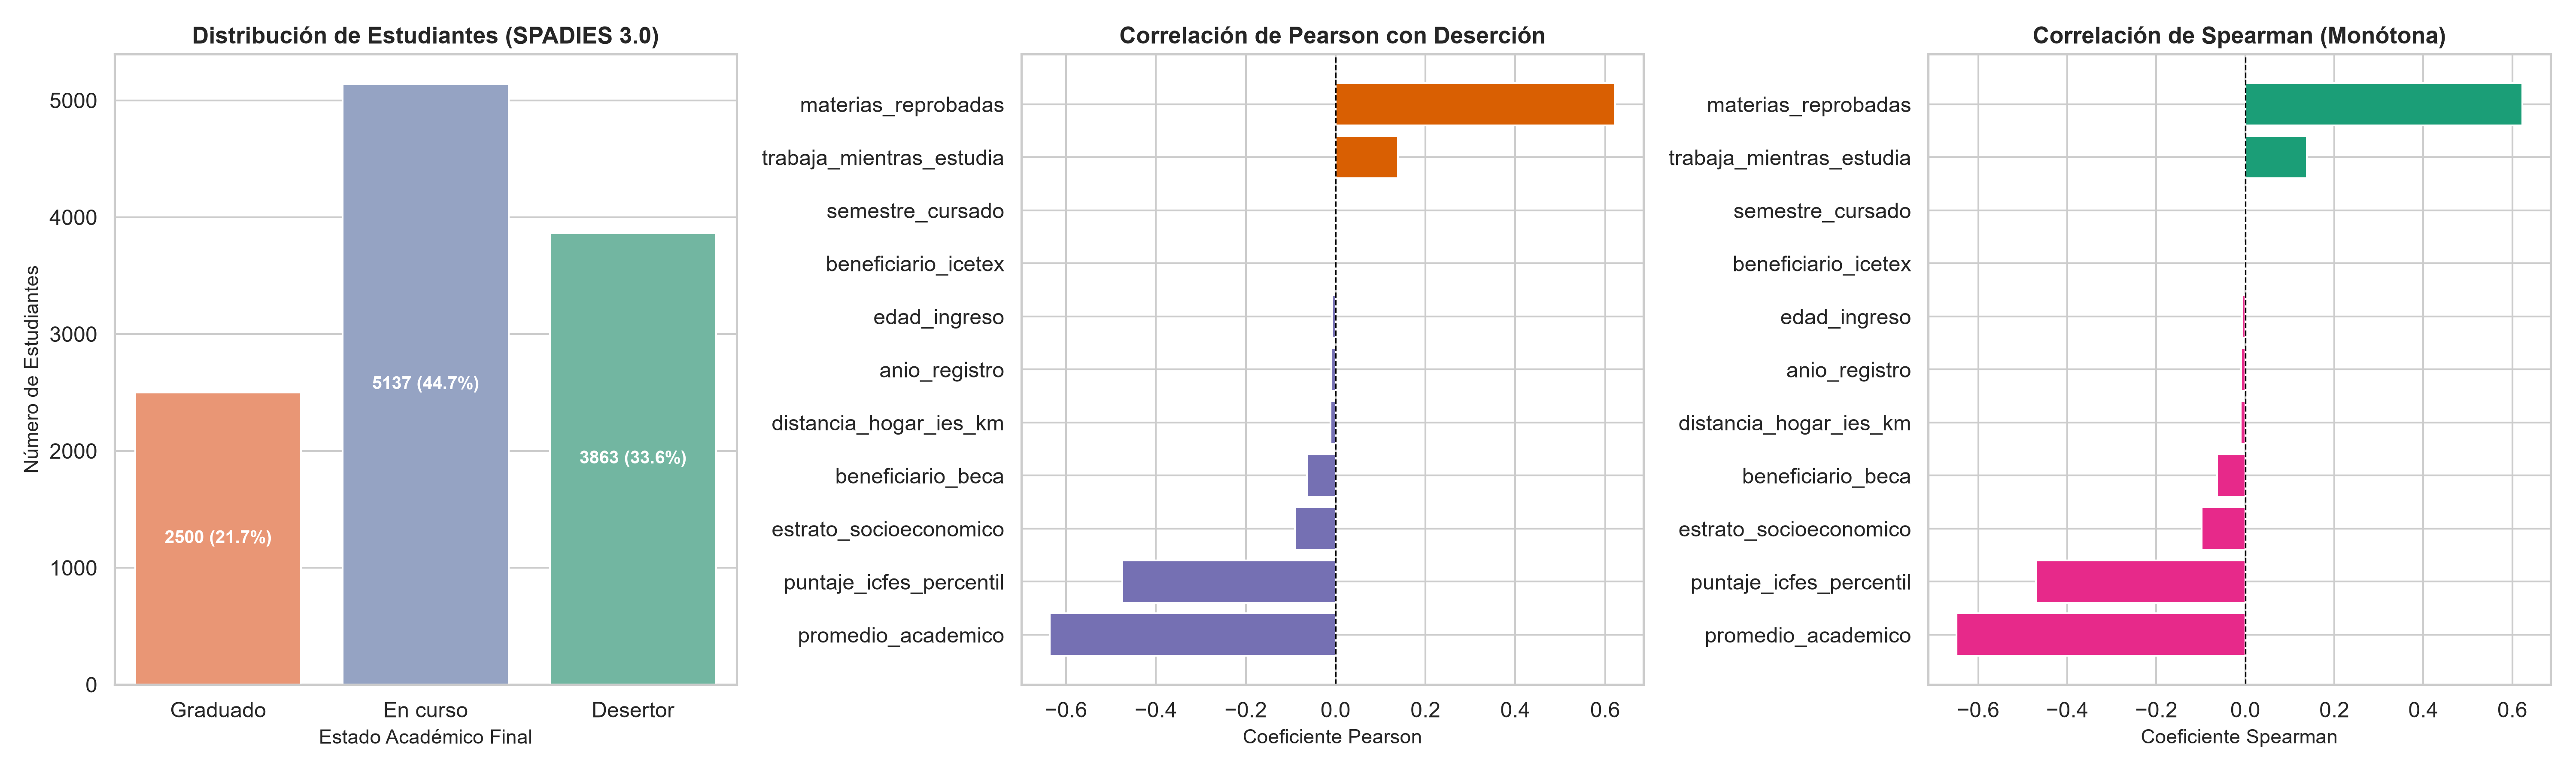
\includegraphics[width=0.98\linewidth]{eda_distribucion_correlaciones.png}\\[0.15cm]
            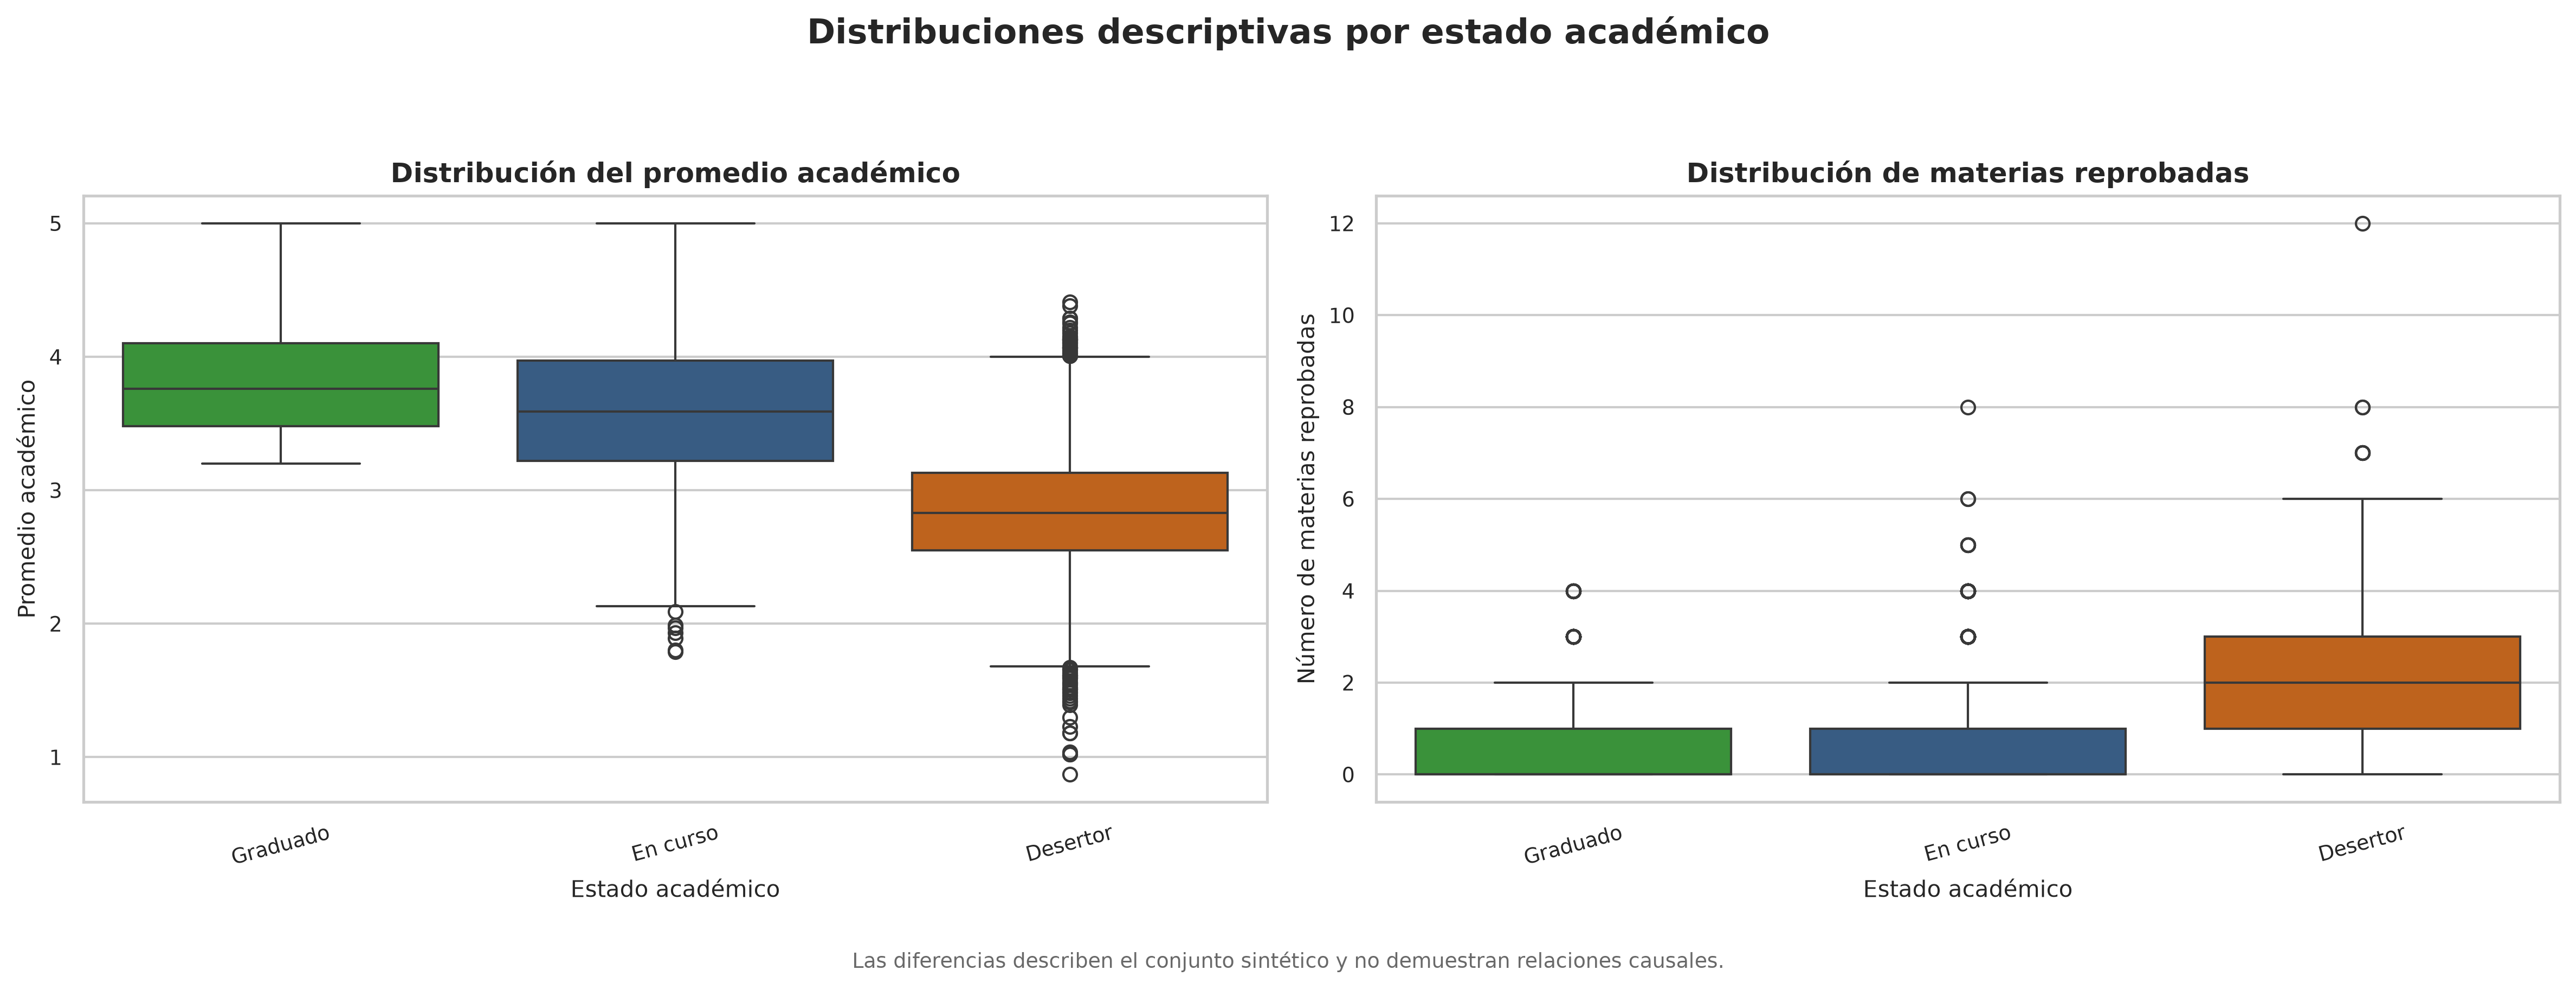
\includegraphics[width=0.88\linewidth]{eda_variables_clave.png}
        \end{column}
    \end{columns}
\end{frame}

% =============================================================
% SLIDE 3: METODOLOGÍA: ROL ESTRUCTURAL DE LA ESCALA
% =============================================================
\begin{frame}{2. Metodología: La Sensibilidad Geométrica de SVM y el Escalado}
    \begin{columns}[T]
        % Columna Izquierda: Formulación
        \begin{column}{0.48\textwidth}
            \begin{block}{\textbf{Dependencia Geométrica del Kernel RBF}}
                \begin{equation*}
                    K(x_i, x_j) = \exp\left(-\gamma \|x_i - x_j\|^2\right)
                \end{equation*}
                \begin{itemize}\small
                    \item Si no se escala, variables con magnitudes amplias dominan la norma euclidiana $\|x_i - x_j\|^2$.
                    \item Caso crítico: \texttt{distancia\_hogar\_ies\_km} ($\text{Skewness} = +5.05$, valores hasta 250 km) apaga al \texttt{promedio\_academico} ($0.0 - 5.0$).
                \end{itemize}
            \end{block}

            \begin{block}{\textbf{Validación Experimental Rigurosa}}
                \begin{itemize}\small
                    \item \textbf{50 Particiones Monte Carlo} independientes (80\% entrenamiento / 20\% prueba estratificada).
                    \item \textbf{Sin fuga de datos (*data leakage*):} Ajuste estricto dentro de un \texttt{Pipeline} de Scikit-Learn.
                \end{itemize}
            \end{block}
        \end{column}

        % Columna Derecha: Efecto de escaladores
        \begin{column}{0.50\textwidth}
            \centering
            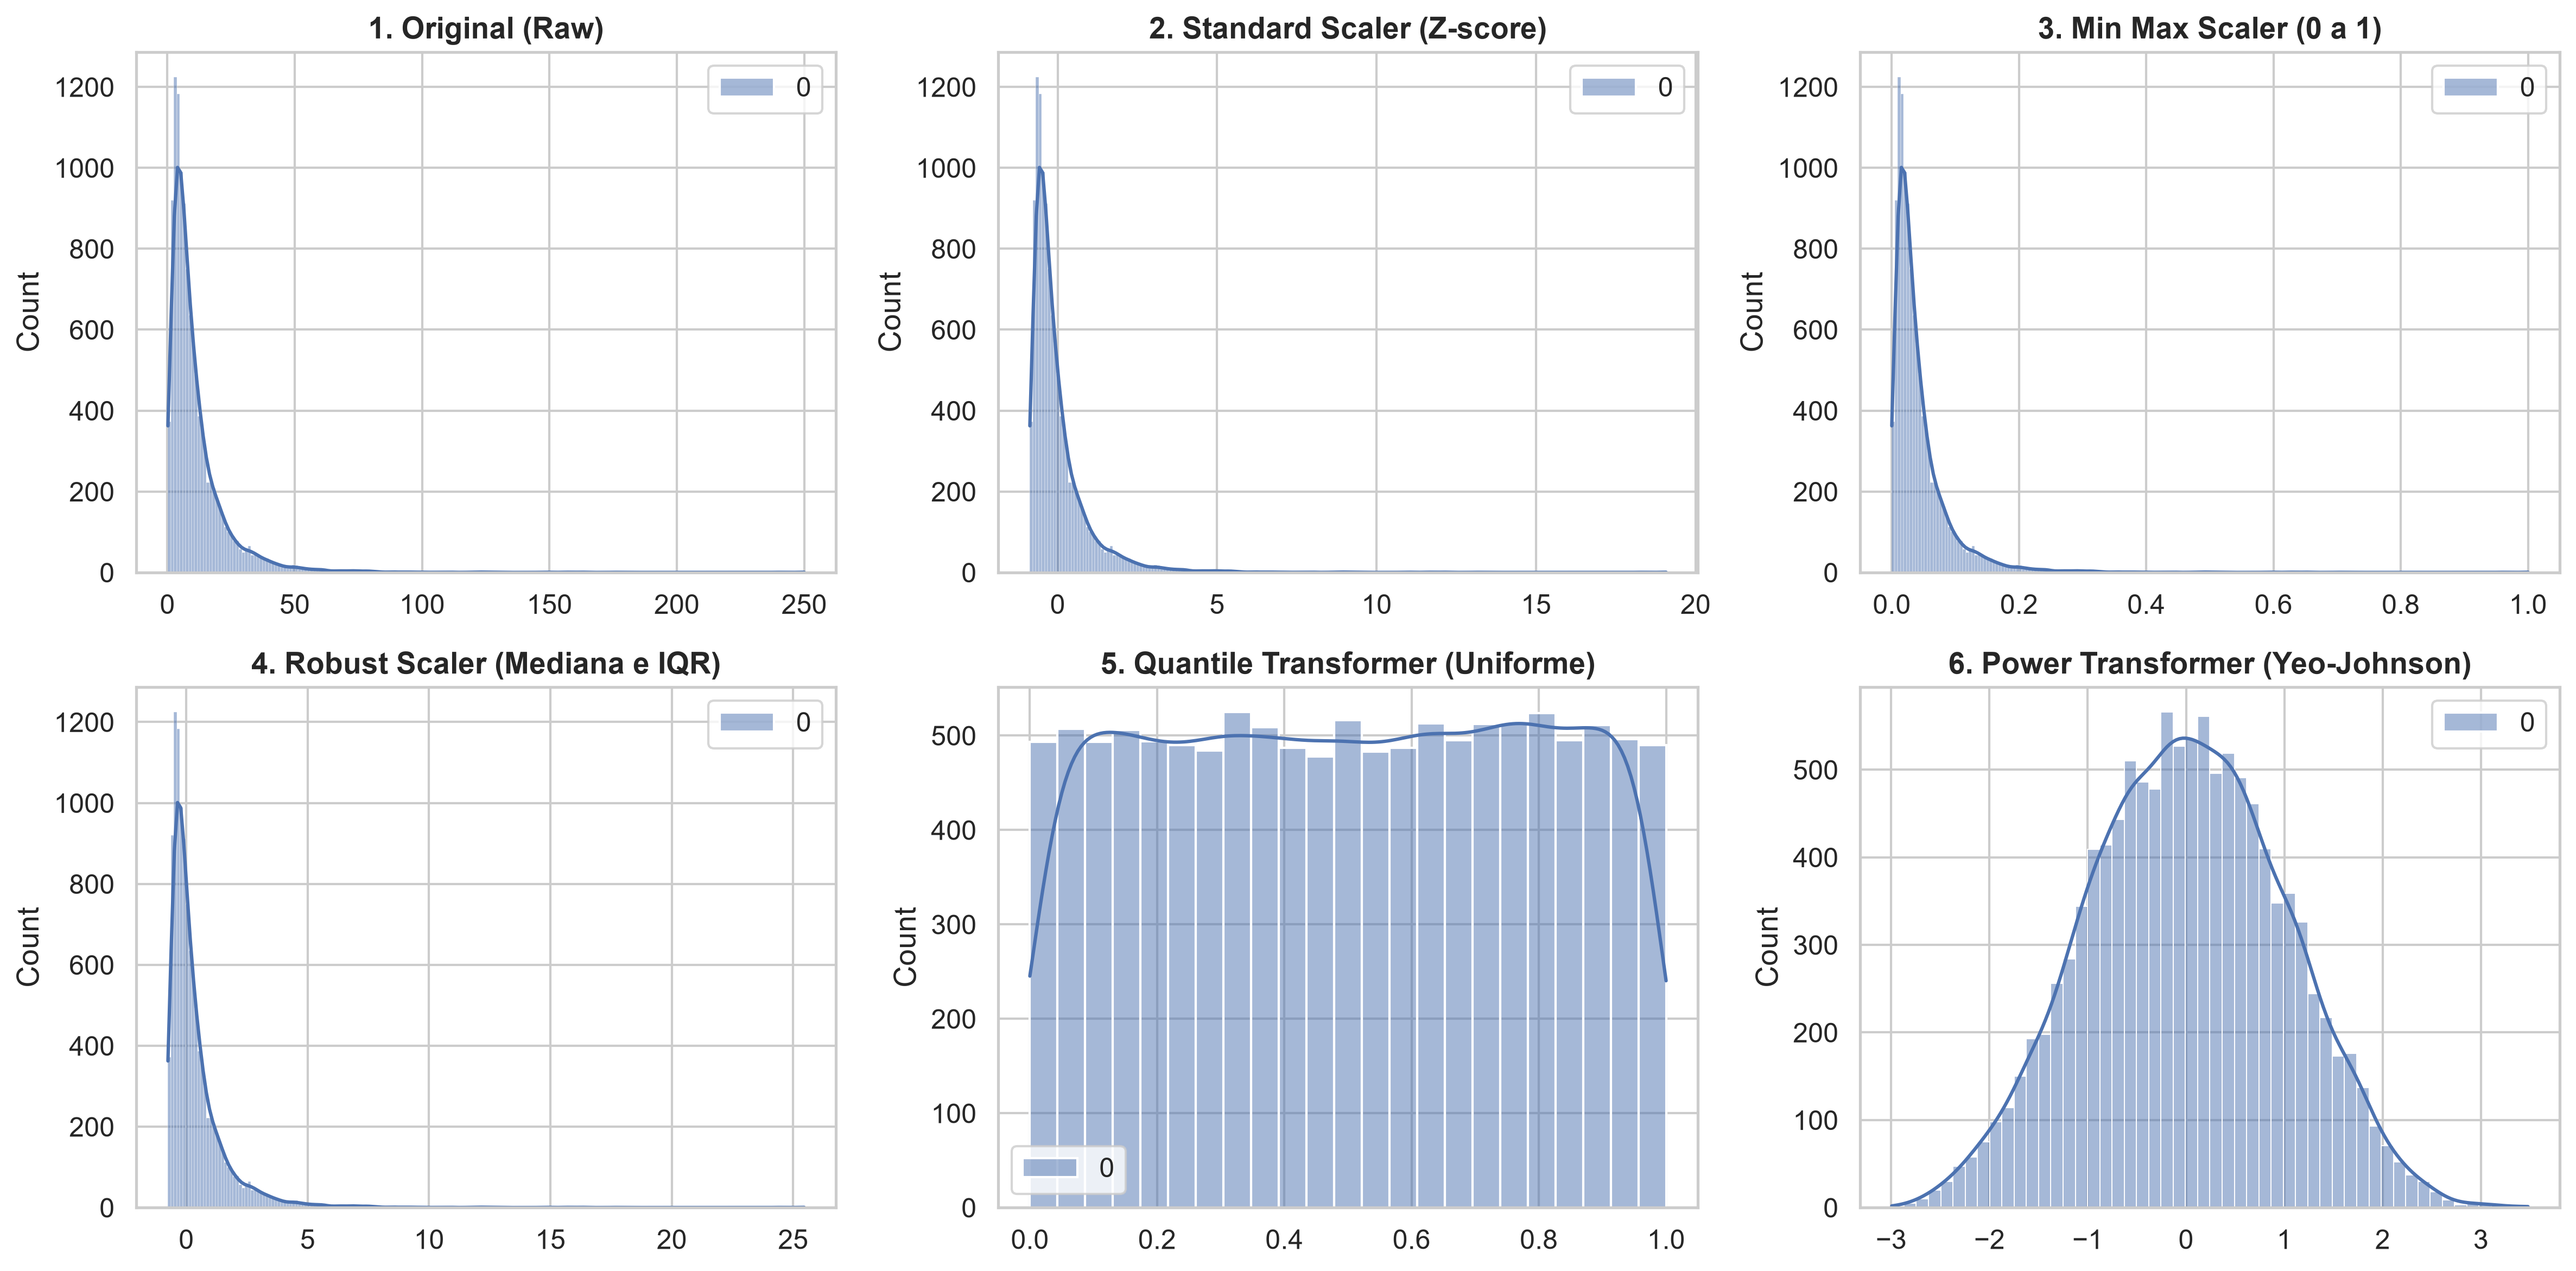
\includegraphics[width=0.98\linewidth]{eda_efecto_escaladores.png}
            \captionof{figure}{\scriptsize Comportamiento de \texttt{distancia\_hogar\_ies\_km} ante 6 transformadores.}
        \end{column}
    \end{columns}
\end{frame}

% =============================================================
% SLIDE 4: RESULTADOS EXPERIMENTALES E INTERPRETABILIDAD
% =============================================================
\begin{frame}{3. Resultados: Ranking de Normalizadores y Frontera Nítida}
    \begin{columns}[T]
        % Columna Izquierda: Ranking
        \begin{column}{0.48\textwidth}
            \centering
            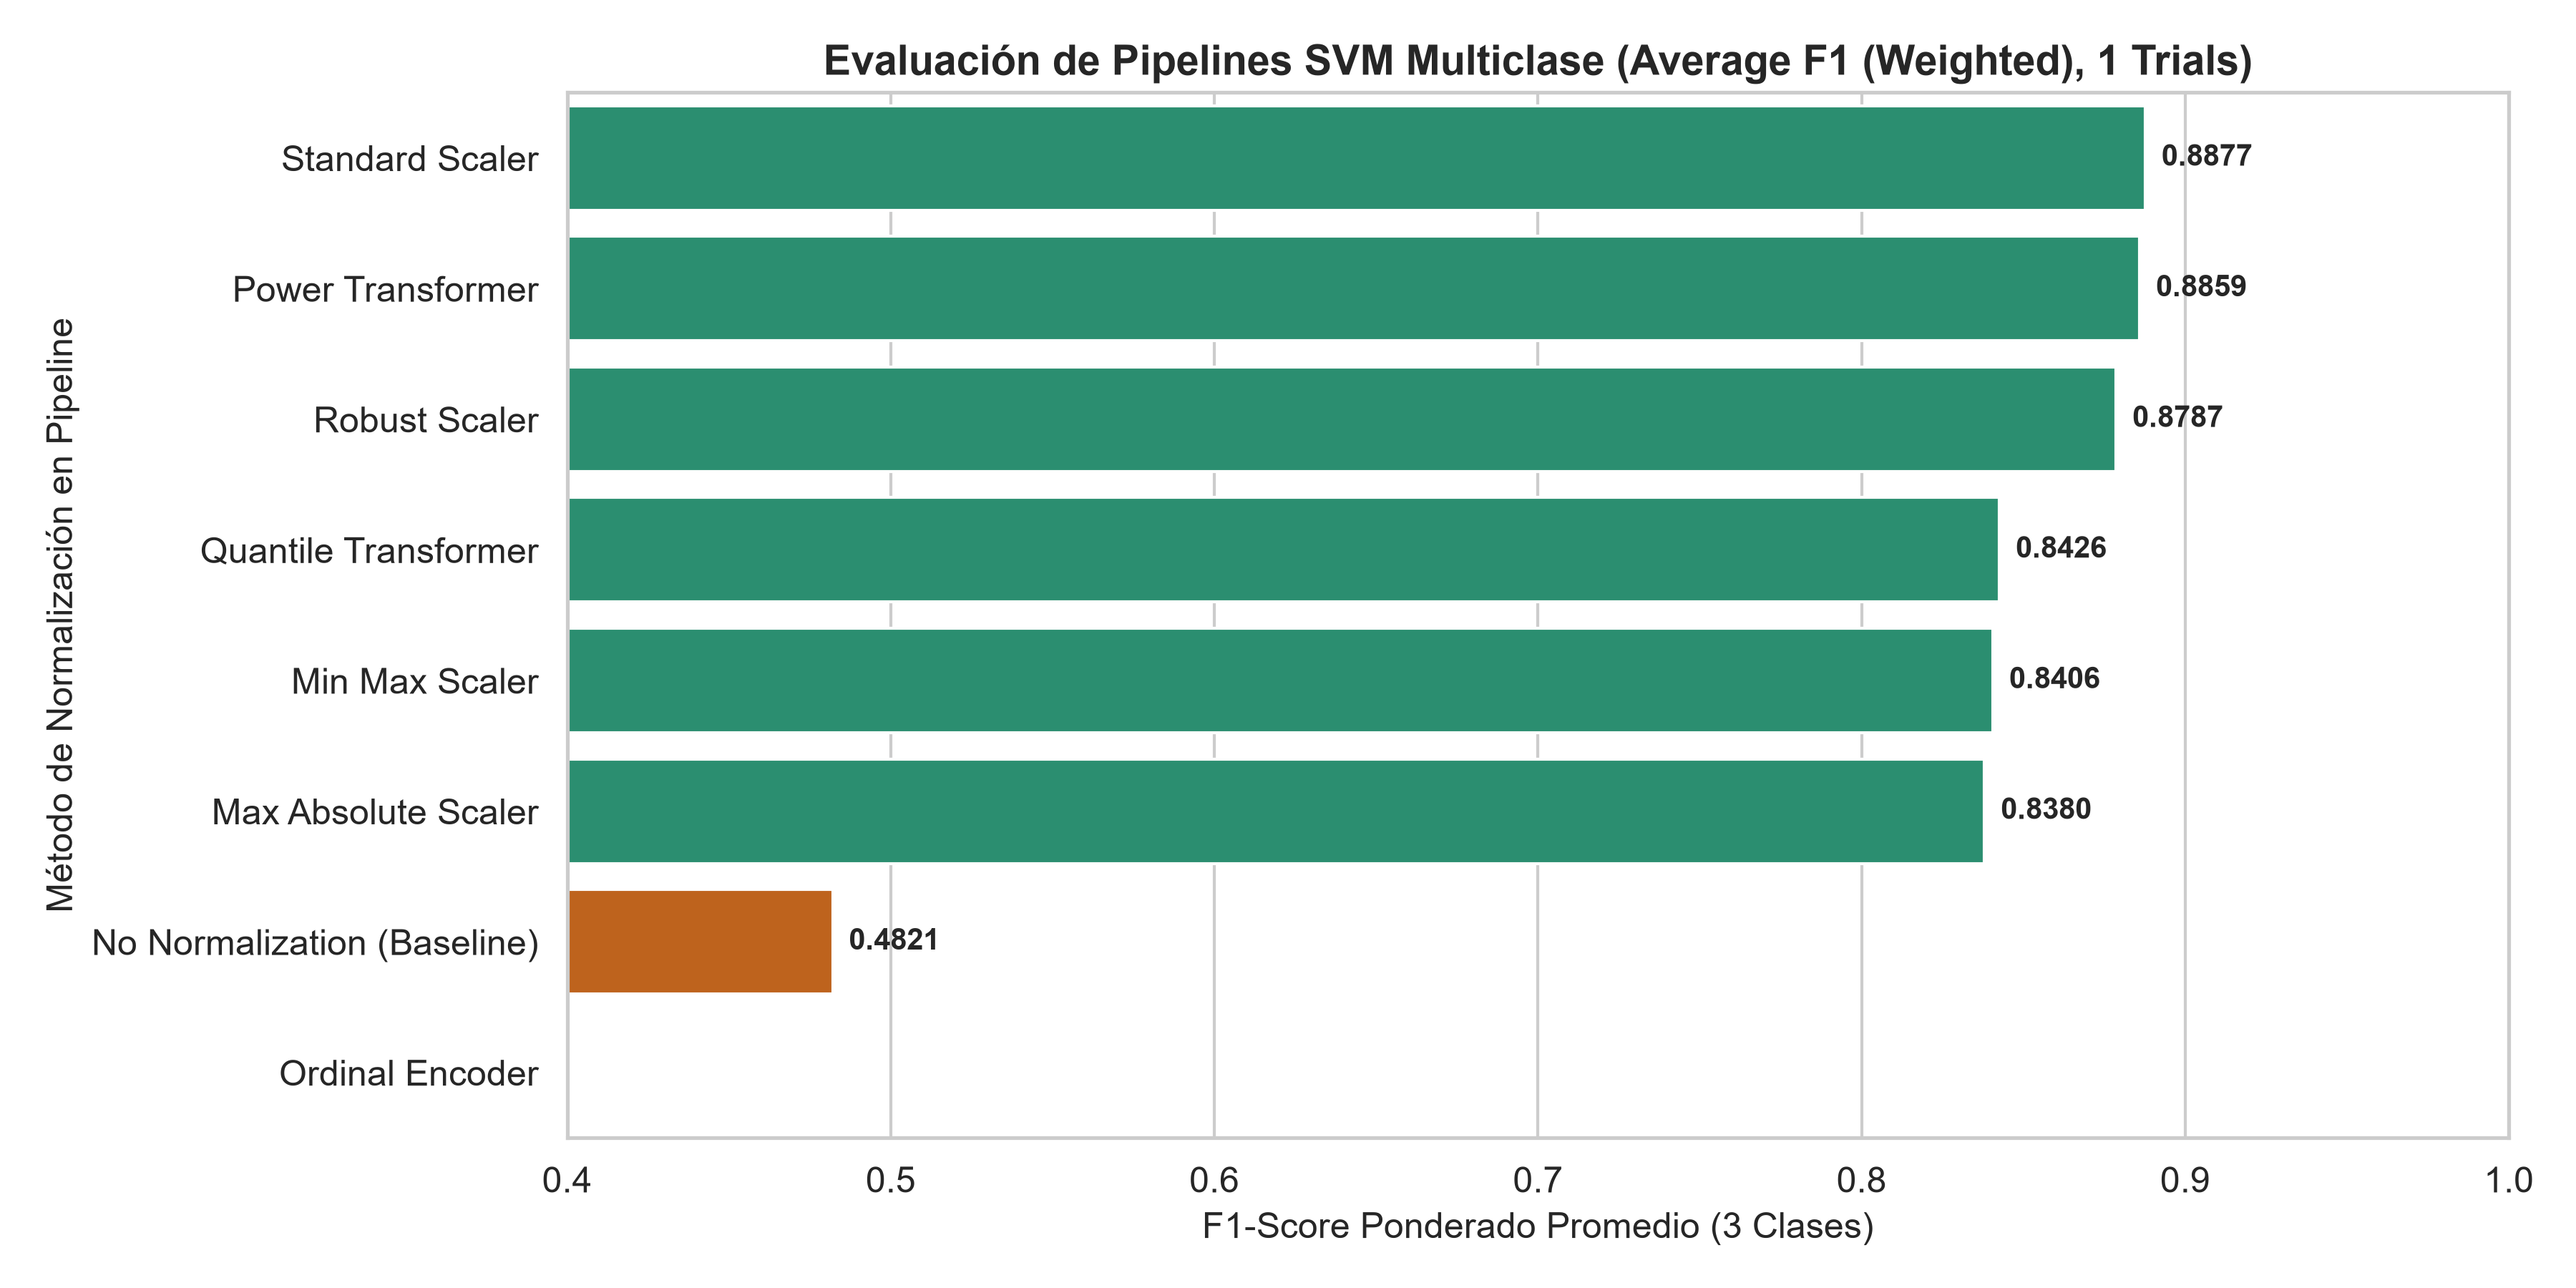
\includegraphics[width=0.98\linewidth]{svm_normalizacion_vs_baseline.png}\\[0.1cm]
            \begin{block}{\textbf{Impacto Cuantitativo (50 Trials)}}
                \begin{itemize}\scriptsize
                    \item \textbf{Colapso Baseline:} $F_1 = 0.4097 \pm 0.006$ (sin escalar).
                    \item \textbf{StandardScaler / Power:} $F_1 = \mathbf{0.8878} \pm 0.006$ ($+85\%$ de mejora, $t > 48.7$, $p < 10^{-6}$).
                    \item \textbf{Recall de Desertores:} $\mathbf{92.11\%}$ (solo $7.89\%$ falsos negativos).
                \end{itemize}
            \end{block}
        \end{column}

        % Columna Derecha: Frontera en variables reales
        \begin{column}{0.50\textwidth}
            \centering
            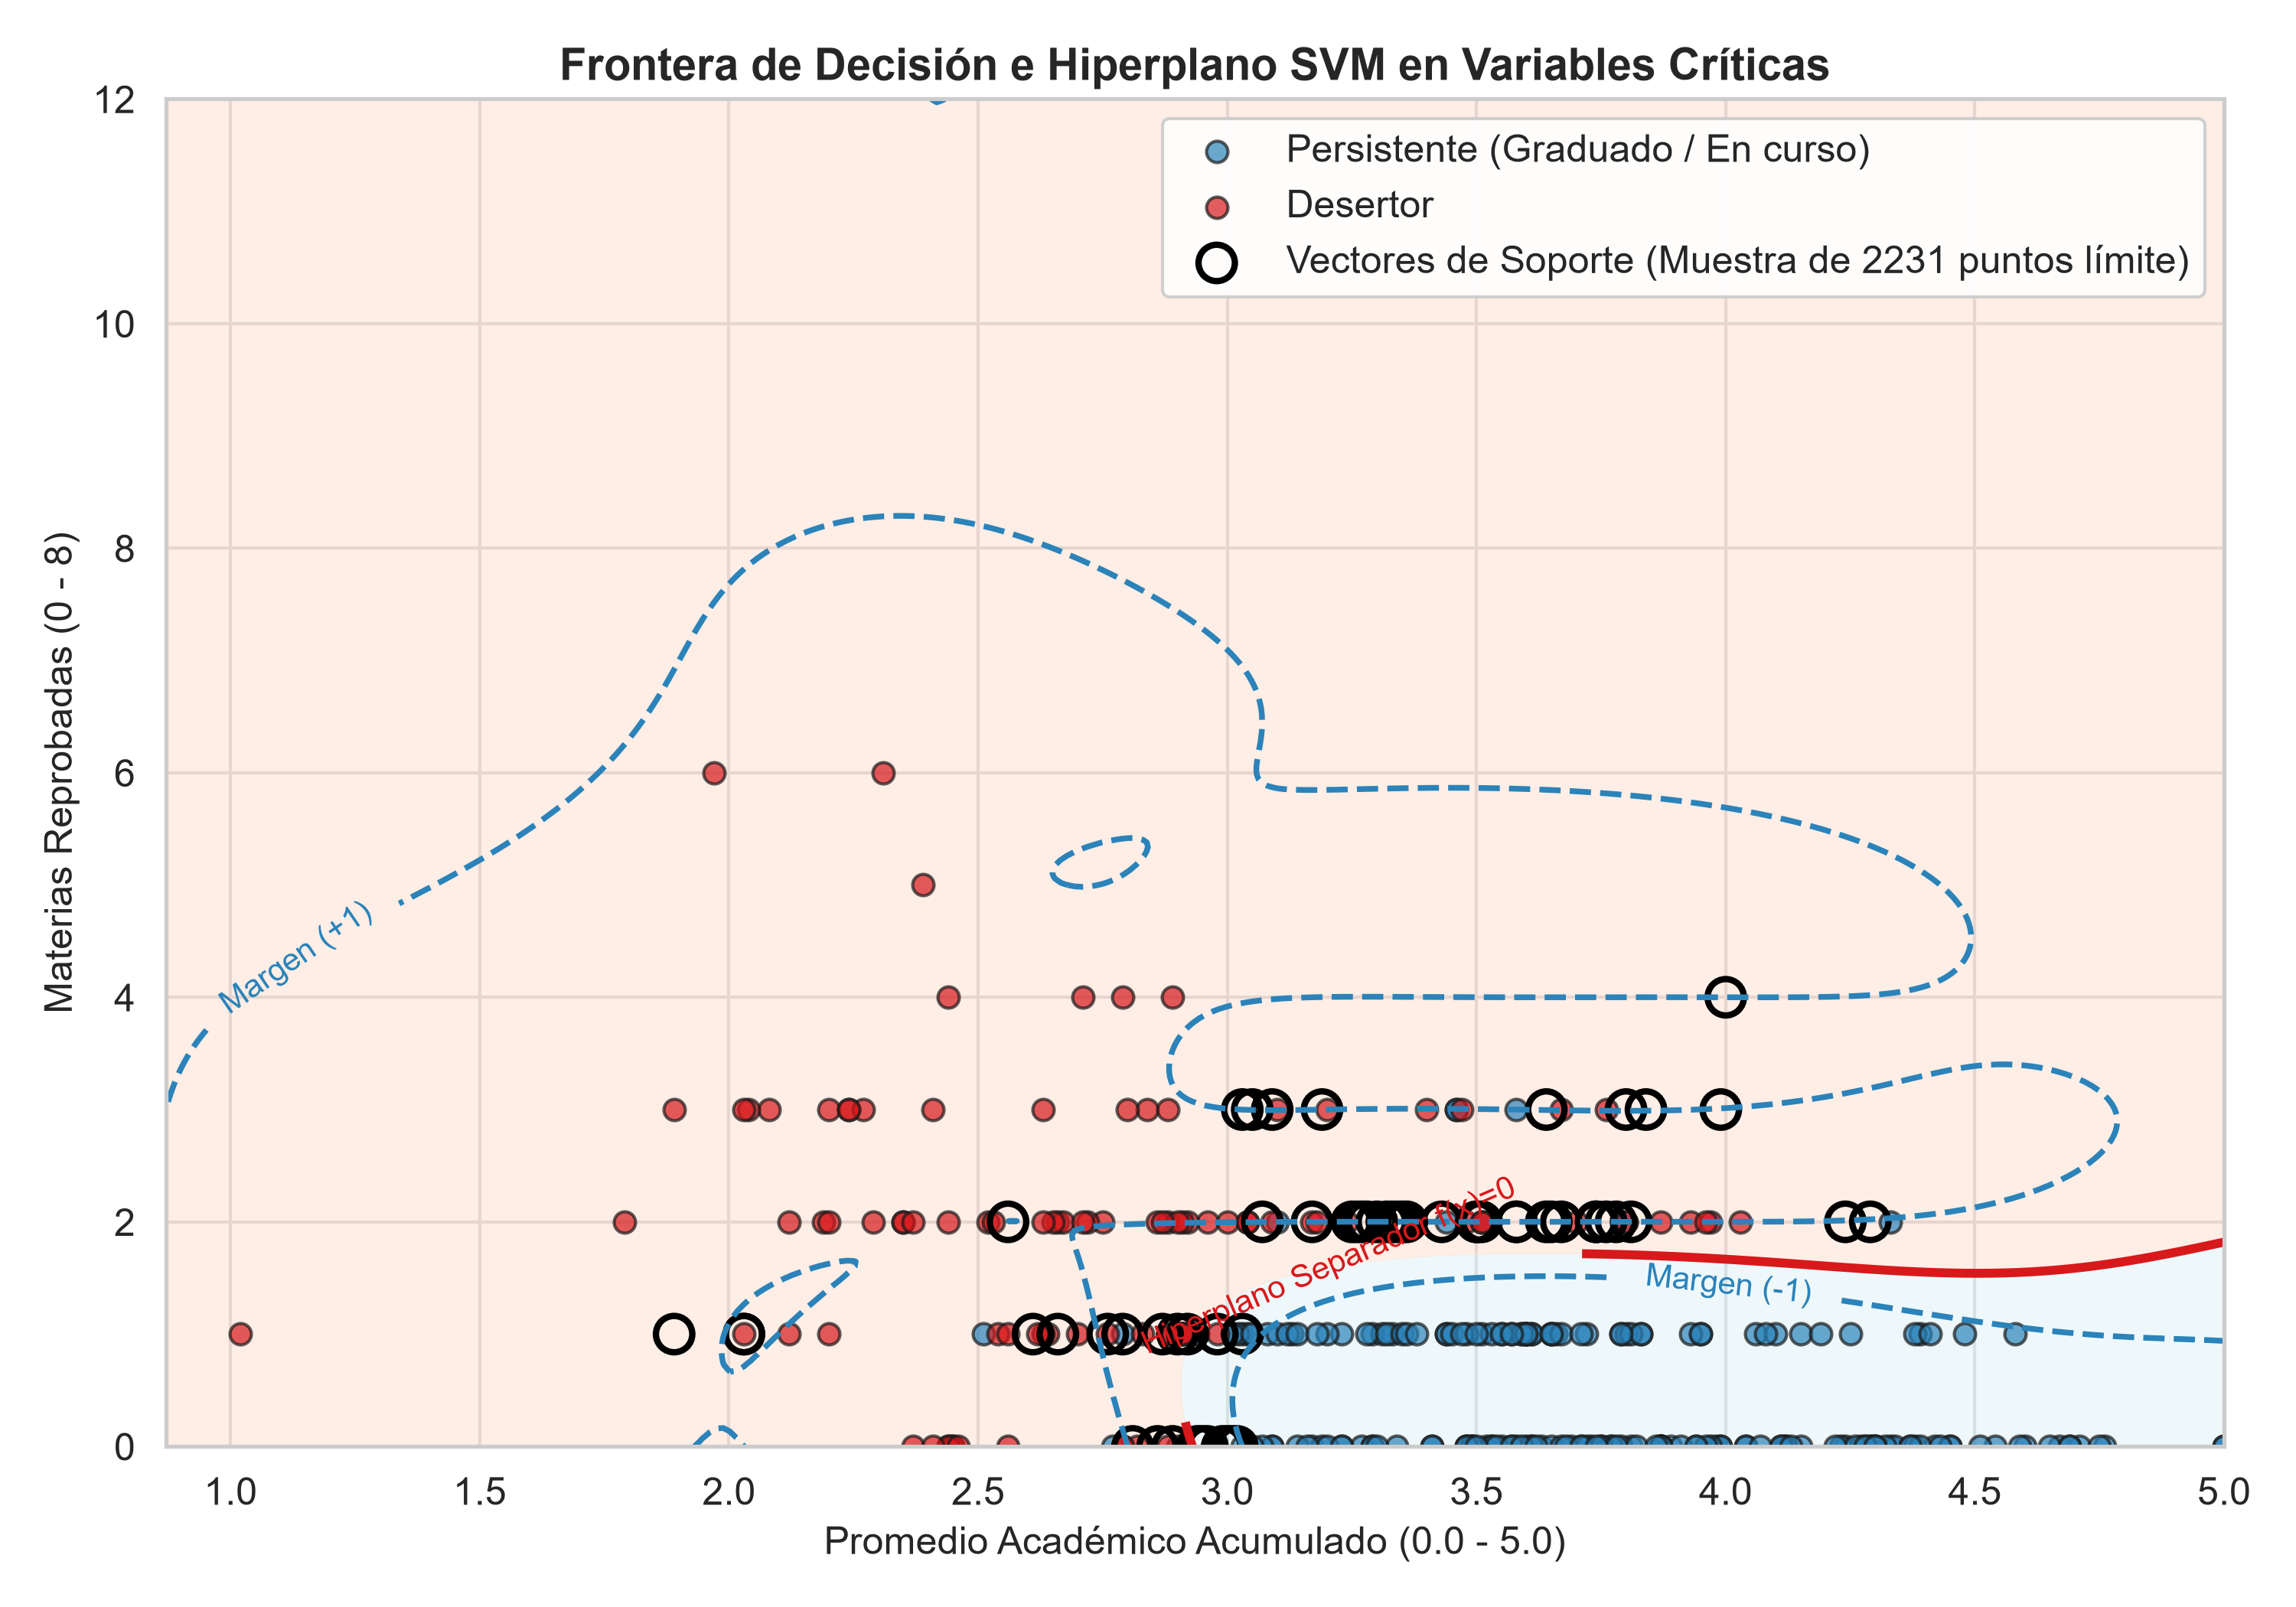
\includegraphics[width=0.95\linewidth]{svm_hiperplano_top2_variables.png}
            \begin{block}{\textbf{Lectura Institucional de la Frontera}}
                \begin{itemize}\scriptsize
                    \item \textbf{Línea roja $f(x)=0$:} Umbral exacto que activa alerta temprana.
                    \item \textbf{Vectores de soporte (halos):} \textbf{Estudiantes en riesgo límite / cuerda floja} (promedio $\sim 3.0$, $1$ o $2$ reprobadas) $\rightarrow$ Máxima prioridad de tutoría.
                \end{itemize}
            \end{block}
        \end{column}
    \end{columns}
\end{frame}

% =============================================================
% SLIDE 5: CONCLUSIONES Y APLICACIÓN INSTITUCIONAL
% =============================================================
\begin{frame}{4. Conclusiones y Aplicación en Bienestar Universitario}
    \begin{columns}[T]
        % Columna Izquierda: Figuras operativas
        \begin{column}{0.48\textwidth}
            \centering
            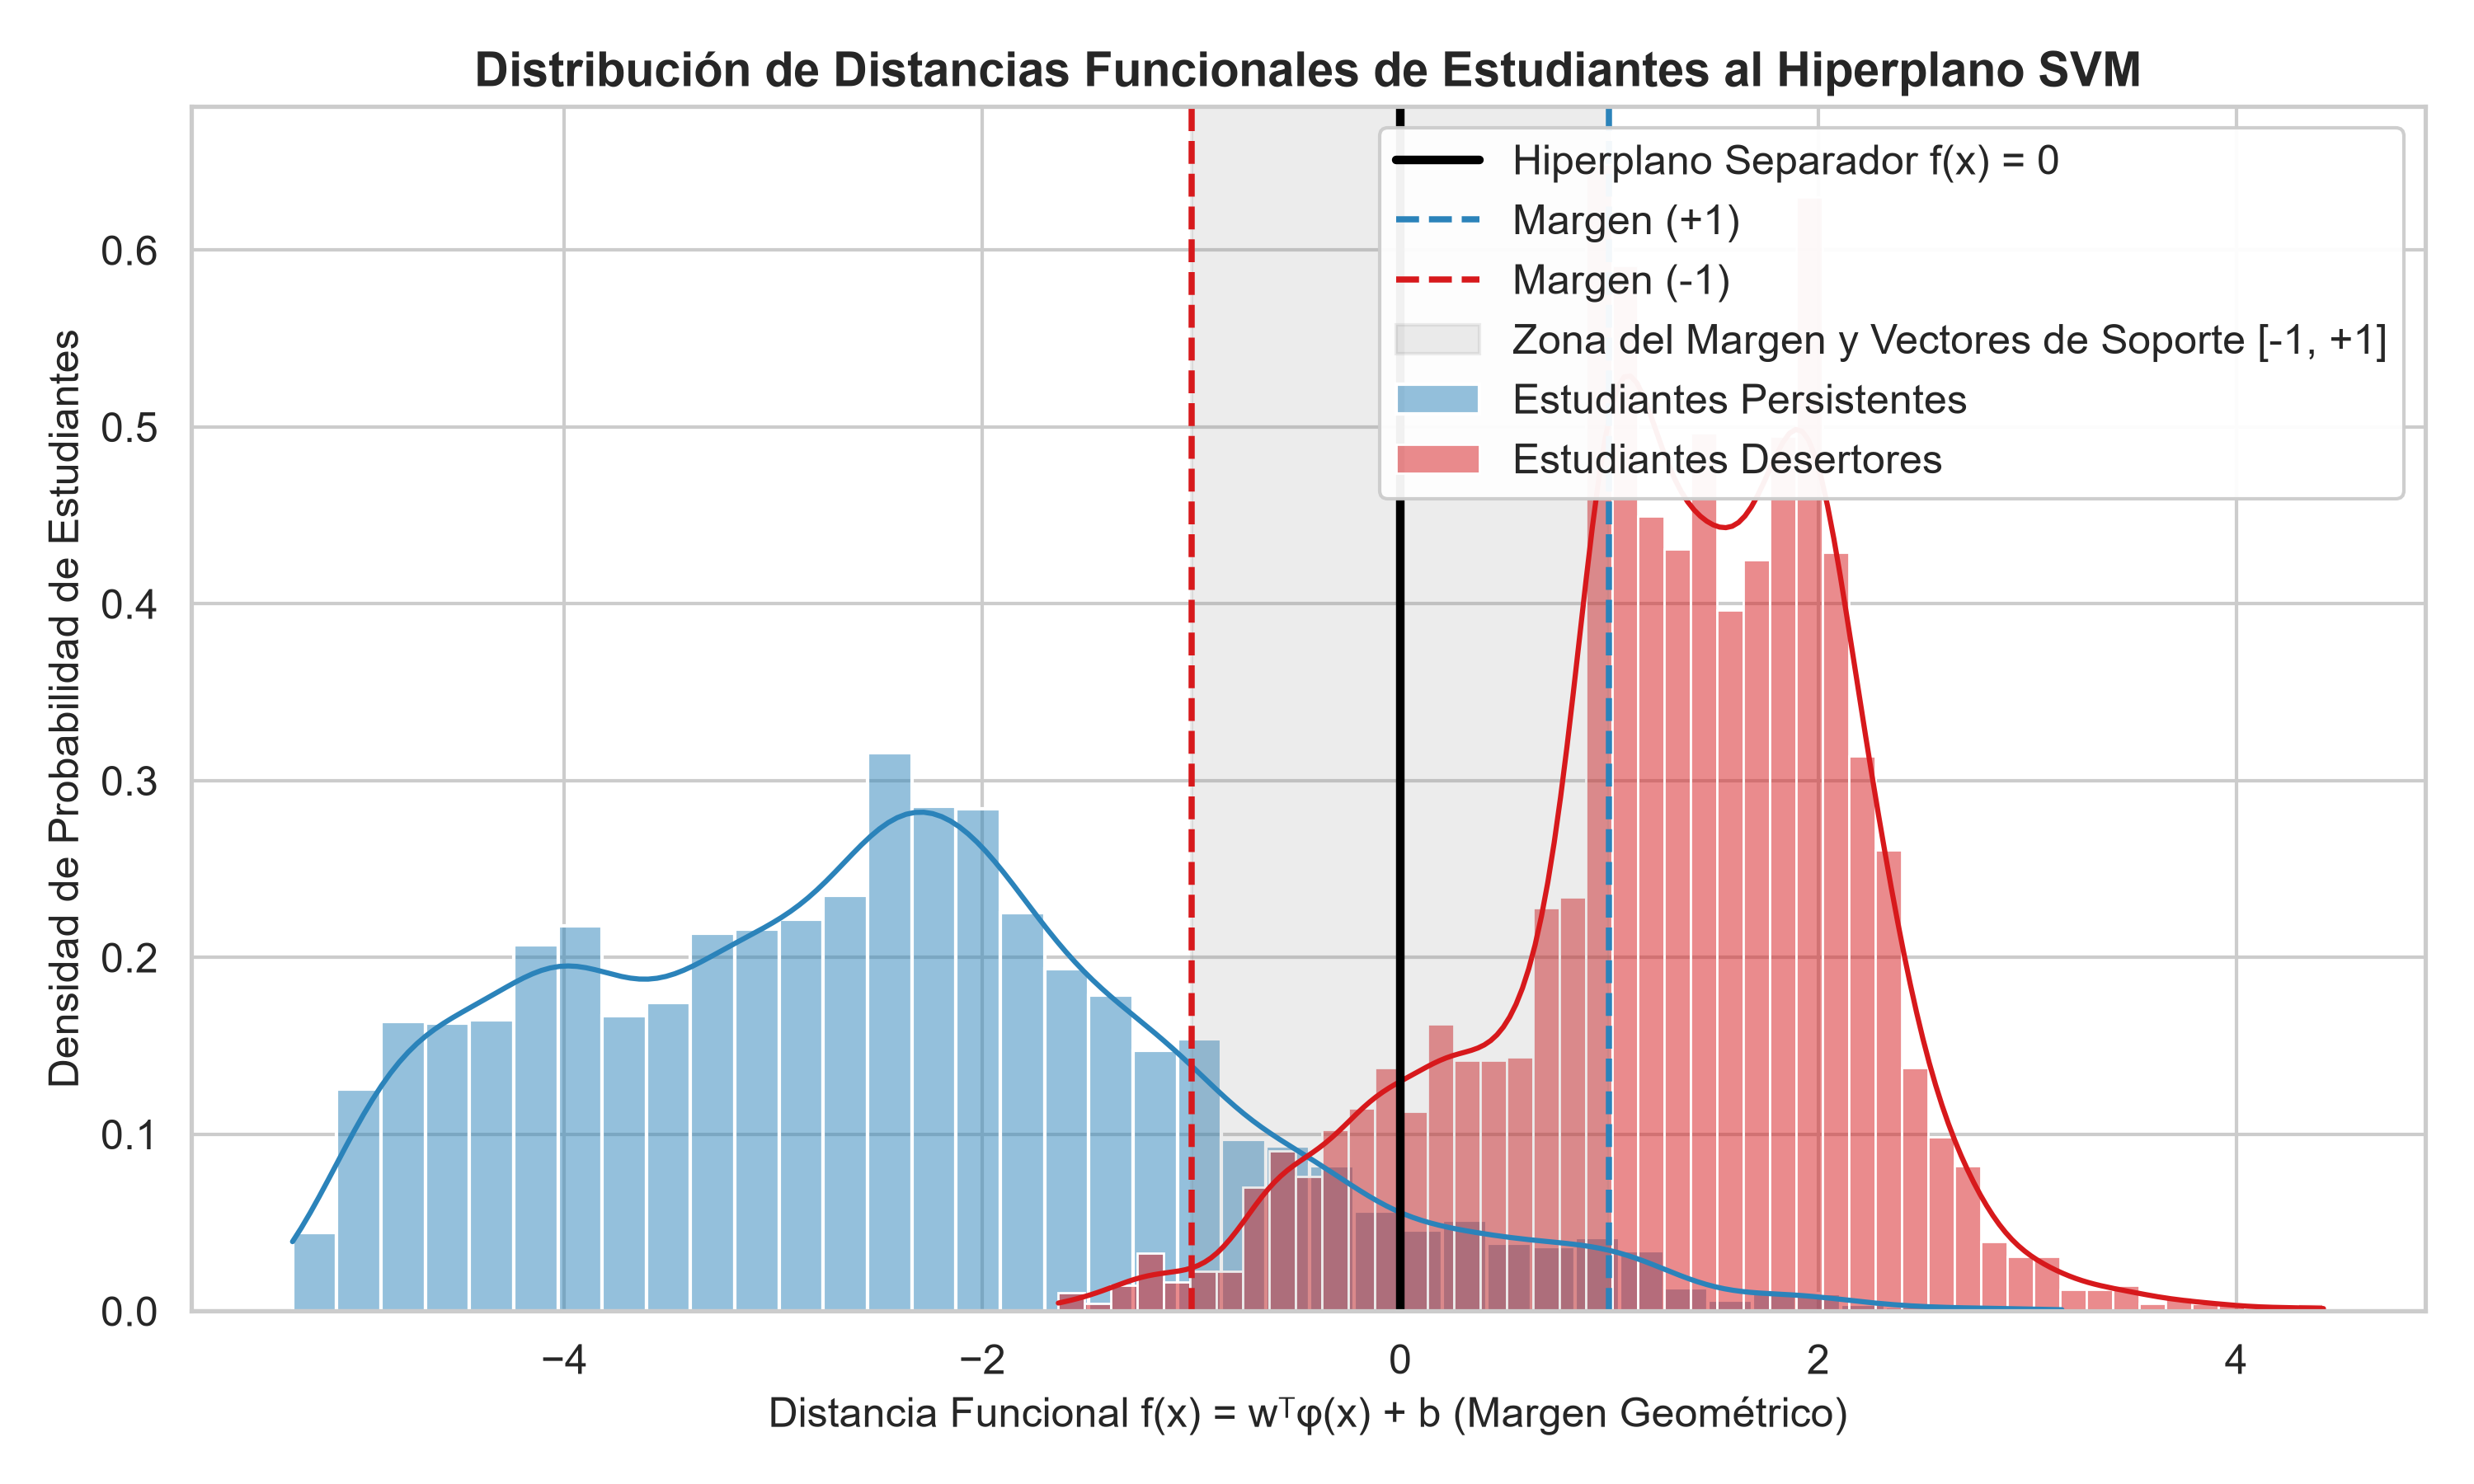
\includegraphics[width=0.92\linewidth]{svm_distancia_hiperplano_estudiantes.png}\\[0.1cm]
            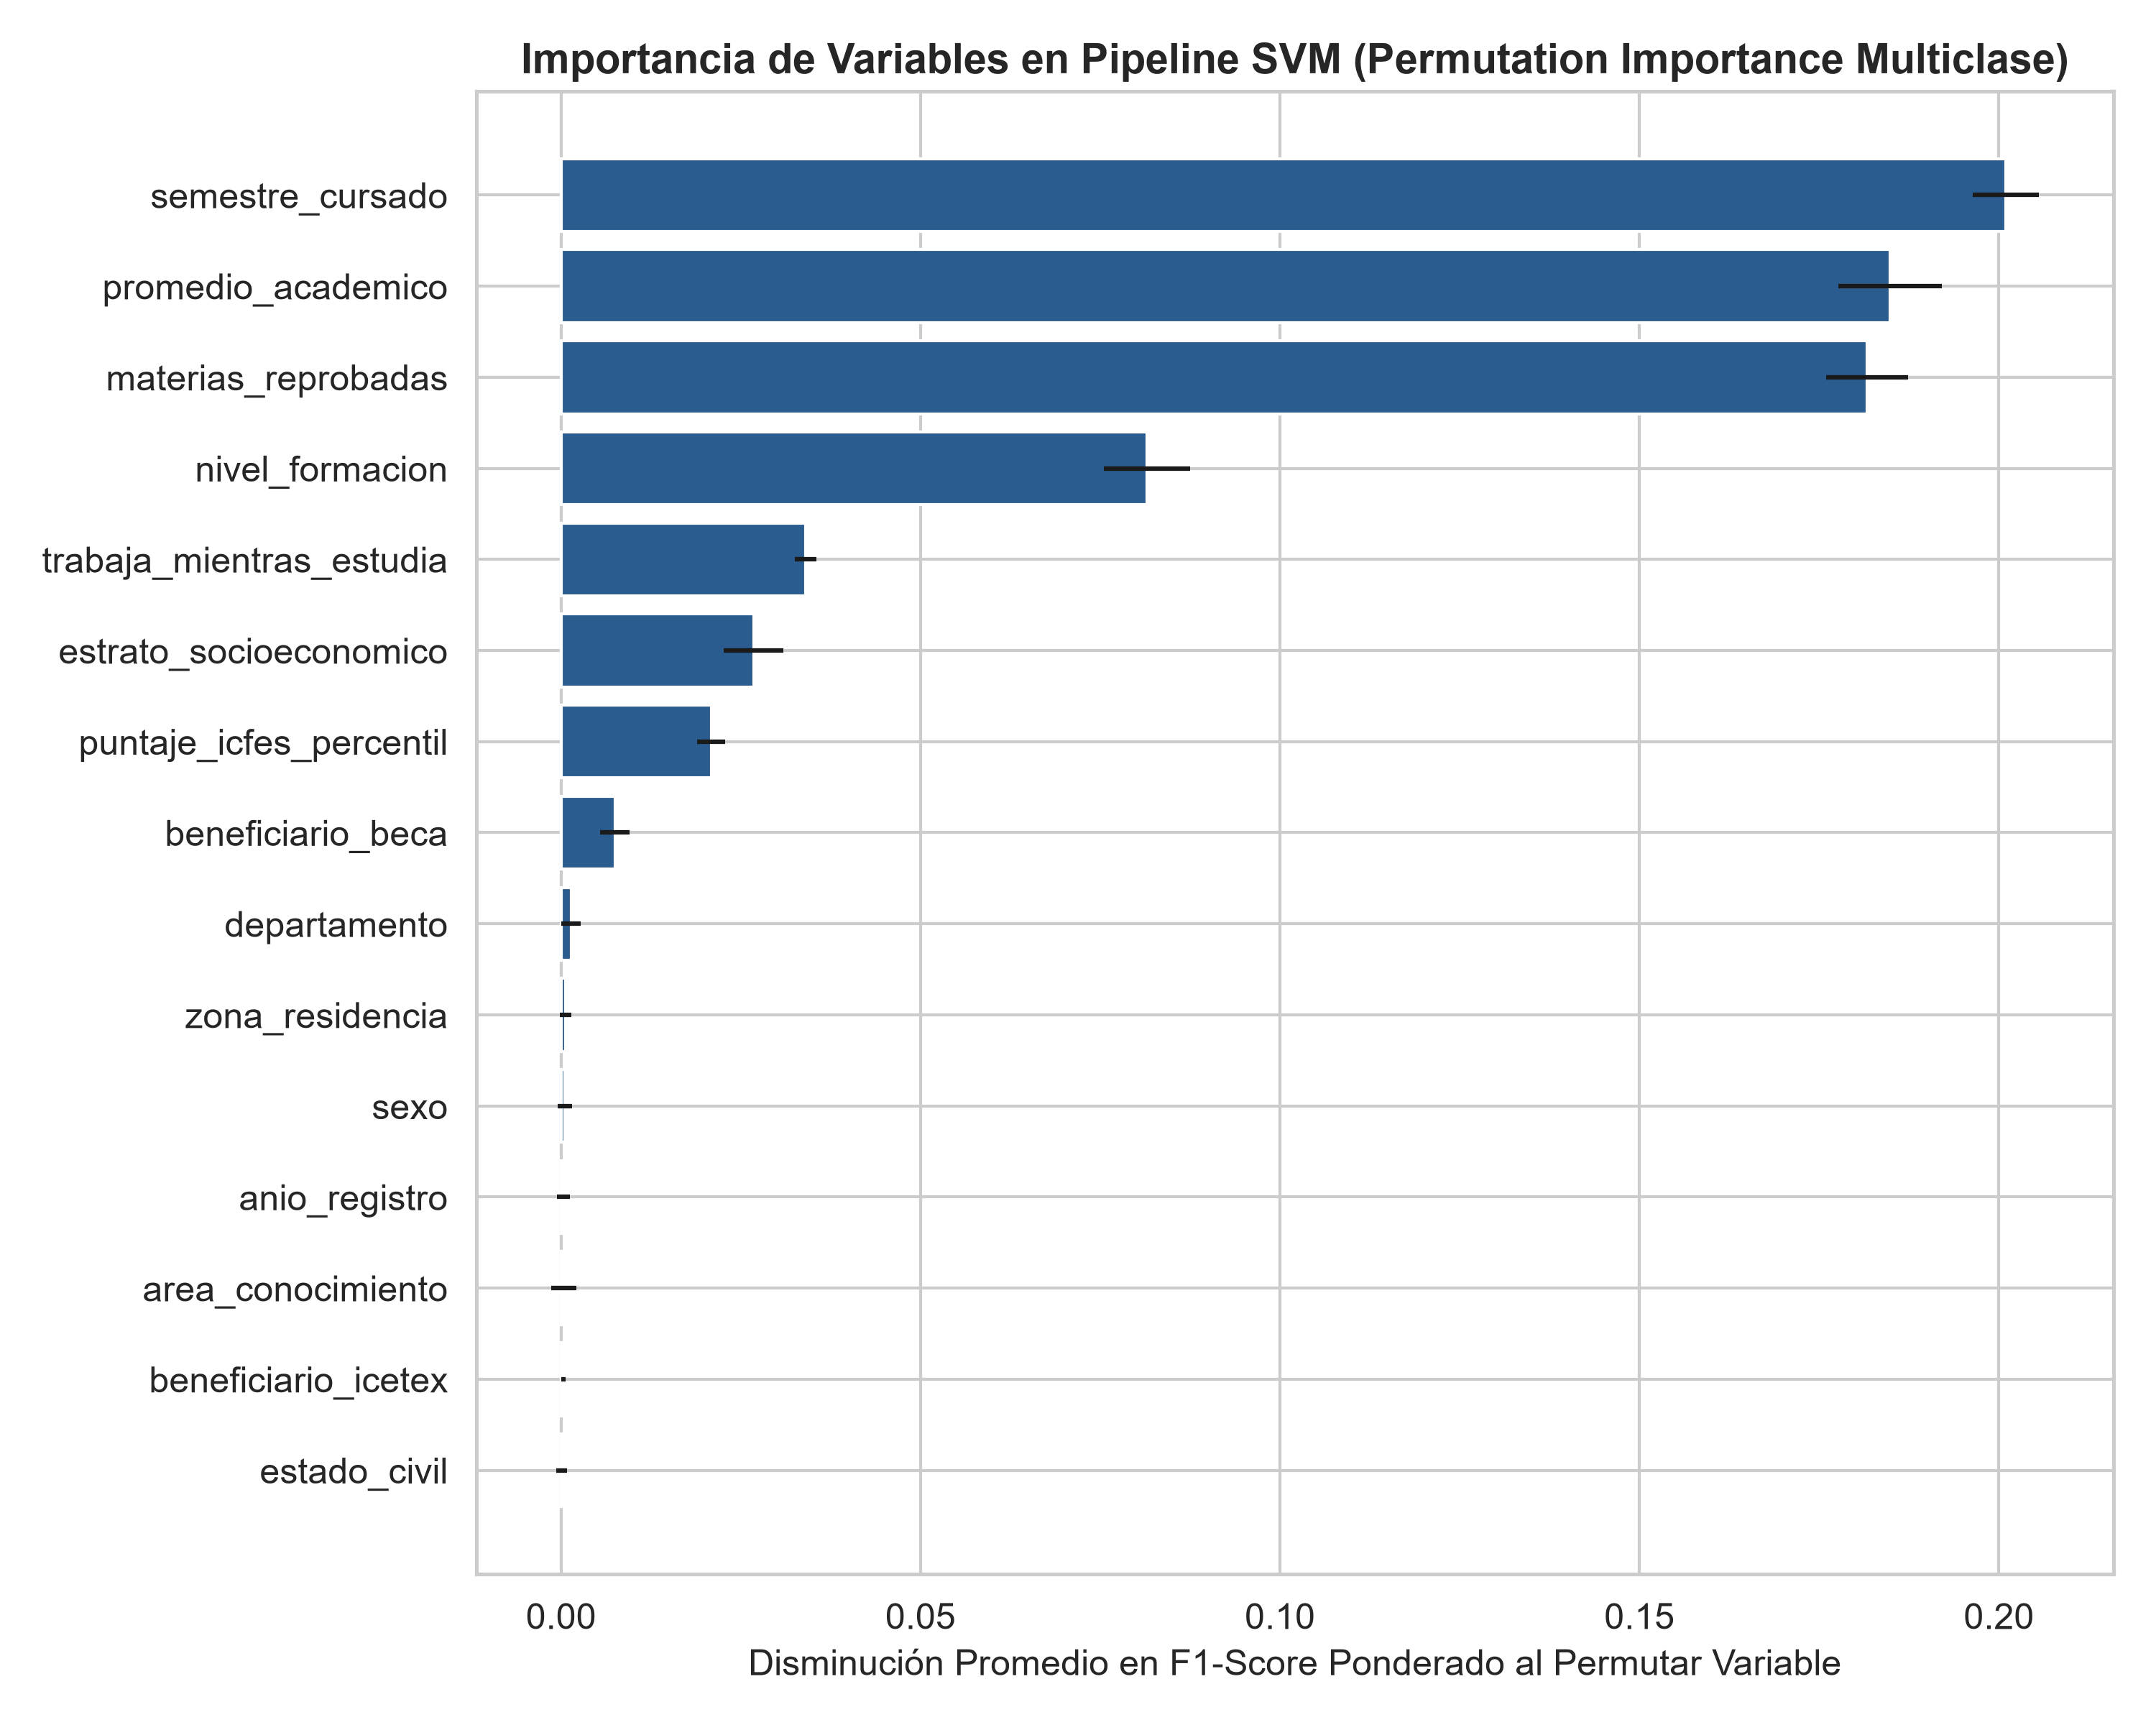
\includegraphics[width=0.92\linewidth]{svm_importancia_variables.png}
        \end{column}

        % Columna Derecha: Conclusiones
        \begin{column}{0.50\textwidth}
            \begin{block}{\textbf{Estratificación del Riesgo con Distancia $f(x)$}}
                \begin{itemize}\scriptsize
                    \item \textbf{Deserción Consolidada ($f(x) < -1$, 28.3\%):} Readmisión y homologación.
                    \item \textbf{Margen Crítico / Vectores de Soporte ($|f(x)| \le 1$, 19.4\%):} \textbf{Foco de Bienestar} para intervención antes de semana 6.
                    \item \textbf{Permanencia Segura ($f(x) > +1$, 52.3\%):} Avance regular.
                \end{itemize}
            \end{block}

            \begin{block}{\textbf{Recomendaciones Clave para la Universidad}}
                \begin{enumerate}\scriptsize
                    \item \textbf{Preprocesamiento Estructural:} La normalización define la existencia del margen en SVM.
                    \item \textbf{Ventana Crítica Temprana:} \texttt{semestre\_cursado} es la variable \#1 ($\Delta F_1 \approx 0.201$); intervenir en semestres 1 a 3.
                    \item \textbf{Auditoría de Equidad (Fairness):} Brecha de detección $< 4\%$ entre subgrupos (sexo, rural/urbano).
                \end{enumerate}
            \end{block}
        \end{column}
    \end{columns}
\end{frame}

\end{document}
